% Lab 9 -- IEEE conference paper skeleton (Task 4). Compile with pdfLaTeX + BibTeX (Overleaf default).
\documentclass[conference]{IEEEtran}
% To switch to ACM: \documentclass[sigconf]{acmart} (and use acmart author/abstract commands; remove IEEEtran blocks).
% One column: \documentclass[conference,onecolumn]{IEEEtran} is not allowed by IEEE; use journal option for testing only.

\usepackage[utf8]{inputenc}
\usepackage[T1]{fontenc}
\usepackage{amsmath,amssymb}   % mathematics
\usepackage{booktabs}          % publication-quality tables
\usepackage{graphicx}          % figures
\usepackage{tikz}              % pipeline diagram
\usetikzlibrary{arrows.meta,positioning,shapes.geometric}
\usepackage{cite}              % sorted, compressed numeric citations [1]--[3]
\usepackage[hidelinks]{hyperref}  % load last (cross-references, URLs)

\newcommand{\Rec}{\mathrm{Rec}}
\newcommand{\FPR}{\mathrm{FPR}}

\begin{document}

\title{Robustness of Text-Based Phishing E-mail Detectors\\to LLM Paraphrasing}

\author{\IEEEauthorblockN{Dias Moldassanov}
\IEEEauthorblockA{Narxoz University\\Almaty, Kazakhstan}
\and
\IEEEauthorblockN{Bilal Samat}
\IEEEauthorblockA{Narxoz University\\Almaty, Kazakhstan}}

\maketitle

\begin{abstract}
Large language models (LLMs) can rewrite a phishing e-mail in fresh wording. We ask whether such paraphrasing lowers the recall of a text-based detector at a fixed false-positive rate. We build a paired experiment: the same 97 phishing e-mails are scored by one detector (TF-IDF with logistic regression) in their original and paraphrased form, and the decision threshold is fixed on original validation data. Recall at a false-positive rate of 1\% is 0.979 for both versions; none of the 97 e-mails is lost (one-sided 95\% upper bound of the lost share: 3.0\%). The mean detector score falls by 0.53, but the threshold is far away. A ceiling effect and a difference in era between the two corpora limit this conclusion. [Draft: Results and Discussion are written in Task~4.]
\end{abstract}

\begin{IEEEkeywords}
phishing detection, large language models, paraphrasing, robustness, reproducibility
\end{IEEEkeywords}

\section{Introduction}
\label{sec:intro}

Phishing remains one of the most costly forms of cybercrime: the FBI Internet Crime Complaint Center report for 2025, as summarised by SpyCloud, puts losses from account takeover, phishing and fraud at USD~20.9 billion~\cite{thies_fbi_2026}. Mail gateways answer this threat with content detectors that score the text of an e-mail and block it above a threshold. Recent work uses classical models, transformers and LLMs for this task~\cite{koide_chatspamdetector_2024,uddin_explainable_2024,thapa_phishing_2025,kuikel_evaluating_2025,ganiuly_trustworthiness_2025}.

The same LLMs help attackers. Heiding et~al.\ show that LLMs can write convincing phishing messages~\cite{heiding_devising_2023} and can run fully automated spear-phishing campaigns that were validated on human subjects~\cite{heiding_evaluating_2024}. An attacker who already owns a working phishing text can therefore ask an LLM for a new wording in seconds, at no cost per variant. A detector that has learned the surface wording of known campaigns may miss such variants.

Among the studies we reviewed, the detection papers report detection quality on fixed test sets, while the attack papers measure human victims or the quality of the generated text. We did not find in this set a paired measurement of how much the recall of a detector falls when the \emph{same} phishing e-mails are rewritten, with the decision threshold held fixed. This is the gap that our study addresses.

We therefore run a controlled paired experiment. Each phishing e-mail is scored in its original and paraphrased form by the same detector, and the threshold is chosen once on original validation data so that only the phishing text differs between the two conditions (Section~\ref{sec:method}).

\subsection{Research Question and Contributions}
\label{sec:intro:rq}

Our research question is:
\begin{description}
  \item[RQ1] Does LLM paraphrasing of phishing e-mails lower the recall of a text-based detector at a fixed false-positive rate of 1\%?
\end{description}
The null hypothesis is that recall does not change; the alternative is that recall decreases. The answer is reported in the results table of Section~\ref{sec:results}. Training with paraphrased e-mails and an analysis by e-mail length were planned as further questions and are left to future work.

The contributions of this paper are:
\begin{itemize}
  \item a paired evaluation protocol with a threshold fixed on original validation data, so that a change in recall can only come from the rewritten text;
  \item a reproducible pipeline from public corpora to figures, with fixed seeds and all result tables in a public repository;
  \item an empirical answer for a TF-IDF and logistic-regression detector: recall at FPR~1\% is unchanged and none of 97 e-mails is lost;
  \item a simple location-shift model of the detector score that predicts the paraphrased recall within 1.2 percentage points without being fitted to it.
\end{itemize}

The rest of the paper is organised as follows. Section~\ref{sec:method} describes the data, the detector, the paraphrasing and the statistics. Results and discussion follow in Sections~\ref{sec:results} and~\ref{sec:discussion}.

\section{Methodology}
\label{sec:method}

\subsection{Data}
\label{sec:method:data}
Phishing e-mails come from Phishing Pot~\cite{peixoto_phishing_pot_2026}, a public collection of 12,865 real e-mails gathered by honeypots. Legitimate e-mails (label~0) come from the CEAS-08 file~\cite{php4life_phishing_dataset}; its spam rows are discarded, because spam is not phishing. We keep English e-mails only and collapse near-duplicate campaigns, which leaves 1,639 phishing and 14,865 legitimate e-mails. Two label giveaways were neutralised in both classes before the split: the anonymiser string of the corpus and four-digit years. The e-mails are split 70/15/15 into training, validation and test sets, stratified by label (11,552 / 2,475 / 2,477 e-mails). The test set holds 246 phishing and 2,231 legitimate e-mails.

\subsection{Problem Formulation}
\label{sec:method:problem}
A detector assigns a score $s(x)$ to an e-mail $x$; a higher score means more phishing-like. An e-mail is flagged if $s(x)>t$. Let $V_0$ be the legitimate validation e-mails, $\alpha=0.01$ the target false-positive rate and $s_{(k)}$ the $k$-th largest score in $V_0$. The threshold is
\begin{equation}
  t \;=\; s_{(\lfloor \alpha |V_0| \rfloor + 1)},
  \label{eq:threshold}
\end{equation}
so that at most $\alpha|V_0|$ legitimate e-mails score above $t$. The threshold is computed once on the original data and reused for every condition. For a set of phishing e-mails $X=\{x_1,\dots,x_n\}$ the primary metric, recall (Eq.~\eqref{eq:recall}), is
\begin{equation}
  \Rec(X) \;=\; \frac{1}{n}\sum_{i=1}^{n}\mathbb{I}\!\left[s(x_i)>t\right].
  \label{eq:recall}
\end{equation}
Let $x_i'$ be the paraphrase of $x_i$. The paired outcome counts
\begin{align}
  b&=\bigl|\{i: s(x_i)>t,\ s(x_i')\le t\}\bigr|,\nonumber\\
  c&=\bigl|\{i: s(x_i)\le t,\ s(x_i')>t\}\bigr|,
  \label{eq:discordant}
\end{align}
the e-mails lost and gained by paraphrasing. The effect of paraphrasing is $\Delta=\Rec(X)-\Rec(X')$. The hypotheses of RQ1 are $H_0\colon \Delta=0$ against $H_1\colon \Delta>0$.

To explain the result we use a location-shift model of the scores. Original phishing scores are modelled as $s\sim\mathcal{N}(\mu,\sigma^2)$, so $\Rec(X)=1-\Phi\bigl((t-\mu)/\sigma\bigr)$, where $\Phi$ is the standard normal distribution function. Paraphrasing shifts the scores by $\delta=\overline{s(x_i')-s(x_i)}$ and leaves $\sigma$ unchanged:
\begin{equation}
  \Rec(X') \;=\; 1-\Phi\!\left(\frac{t-\mu-\delta}{\sigma}\right).
  \label{eq:shift}
\end{equation}
The prediction of Eq.~\eqref{eq:shift} is compared with the measured recall; it is not fitted to it.

\subsection{Detector and Paraphrasing}
\label{sec:method:pipeline}
Fig.~\ref{fig:pipeline} shows the pipeline. The detector is TF-IDF with logistic regression, trained on original training e-mails only; its settings are listed in Table~\ref{tab:params}. The detector is deterministic, so the five seeds give identical numbers; uncertainty is therefore reported by the statistics of Section~\ref{sec:method:stats}.

\begin{figure}[t]
\centering
\resizebox{\columnwidth}{!}{%
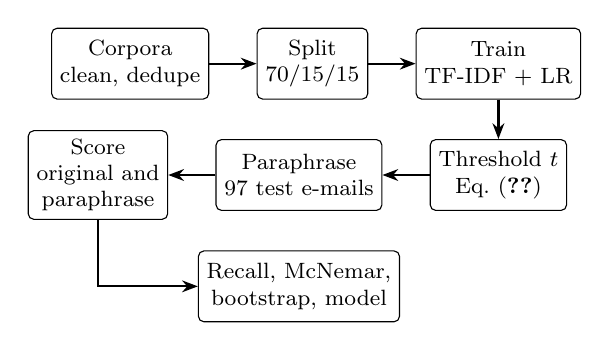
\begin{tikzpicture}[
  node distance=5mm and 6mm,
  box/.style={draw, rounded corners=2pt, align=center, font=\footnotesize, minimum height=9mm, inner sep=3pt},
  arr/.style={-{Stealth[length=2mm]}, thick}]
  \node[box] (clean) {Corpora\\clean, dedupe};
  \node[box, right=of clean] (split) {Split\\70/15/15};
  \node[box, right=of split] (train) {Train\\TF-IDF + LR};
  \node[box, below=of train] (thr) {Threshold $t$\\Eq.~\eqref{eq:threshold}};
  \node[box, left=of thr] (para) {Paraphrase\\97 test e-mails};
  \node[box, left=of para] (score) {Score\\original and\\paraphrase};
  \node[box, below=of para] (stat) {Recall, McNemar,\\bootstrap, model};
  \draw[arr] (clean)--(split);
  \draw[arr] (split)--(train);
  \draw[arr] (train)--(thr);
  \draw[arr] (thr)--(para);
  \draw[arr] (para)--(score);
  \draw[arr] (score)|-(stat);
\end{tikzpicture}}
\caption{Experimental pipeline. The threshold is fixed on original validation data before the paraphrases are scored.}
\label{fig:pipeline}
\end{figure}

The planned paraphraser (Qwen2.5-1.5B-Instruct) could not run in our environment. Instead, 97 phishing e-mails of the test split were paraphrased by an LLM (Claude) with one fixed instruction: keep the meaning, the links and the addresses, and change the wording and the sentence structure. The e-mails are a random sample (seed~0) of the 111 test phishing e-mails of 160 to 900 characters; three explicit adult e-mails were skipped. A paraphrase is accepted if its length is 0.5 to 1.5 times the original and all links are kept; all 97 passed. Our conclusions therefore concern short e-mails and one paraphrasing LLM.

\begin{table}[t]
\caption{Parameters of the experiment.}
\label{tab:params}
\centering
\small
\begin{tabular}{@{}p{0.60\columnwidth}p{0.34\columnwidth}@{}}
\toprule
Parameter & Value \\
\midrule
Target FPR $\alpha$ (validation ham) & 0.01 \\
Guardrail: realised FPR & $\le 0.02$ \\
TF-IDF: features; n-grams; tf & 50,000; 1--2; sublinear \\
Logistic regression & $C=4$, 1000 iter. \\
Seeds & 42--46 \\
Paired test e-mails $n$ & 97 \\
Bootstrap resamples & 10,000 \\
Confidence level & 95\% \\
\bottomrule
\end{tabular}
\end{table}

\subsection{Statistics}
\label{sec:method:stats}
We test $H_0$ with the one-sided exact McNemar test on the discordant pairs $b$ and $c$ of Eq.~\eqref{eq:discordant}. When $b=0$, the one-sided 95\% upper bound of the lost share is the Clopper--Pearson bound. Recall over e-mails is given with a 95\% Wilson interval, and the score shift $\delta$ with a paired bootstrap interval. Outliers are flagged by the interquartile-range rule but not removed. Realised FPR is tracked as a guardrail and must stay below 2\%; it is reported, never filtered. Seeds, library versions and all scripts are in the public repository\footnote{\url{https://github.com/Dias-M/ResearchMetod-MoldassanovDias-BilalSamat}}.

\section{Results}
\label{sec:results}
% Task 4: results table (recall, lost/gained, score shift), Fig.~1--3 from the repository (reports/figures/).
\emph{Draft placeholder: the results are written in Task~4.}

\section{Discussion}
\label{sec:discussion}
% Task 4: interpretation (ceiling effect, era confound), limitations, conclusion.
\emph{Draft placeholder: the discussion is written in Task~4.}



\bibliographystyle{IEEEtran}
\bibliography{references}

\end{document}
